\section{Architektura MySQL}

\subsection{Obsługa połączeń i wątków}
Serwer MySQL oczekuje na połączenia klientów na wielu interfejsach sieciowych:
\begin{itemize}
\item jeden wątek obsługuje połączenia TCP/IP (standardowo port 3306)
\item w systemach UNIX, ten sam wątek obsługuje połączenia poprzez pliki gniazda
\item w systemie Windows osobny wątek obsługuje połączenia komunikacji międzyprocesorowej
\item w każdym systemie operacyjnym, dodatkowy interfejs sieciowy może obsługiwać połączenia administracyjne. Do tego celu może być wykorzystywany osobny wątek lub jeden z wątków menadżera połączeń.
\end{itemize}

Jeżeli dany system operacyjny nie wykorzystuje połączeń na innych wątkach, osobne wątki nie są tworzone.

Maksymalna ilość połączeń zdefinowana jest poprzez zmienną systemową \underline{max\_connections}, który domyślnie przyjmuje wartość 151. Dodaktowo MySQL jedno połączenie rezerwuje dla użytkownika z uprawnieniami \underline{SUPER} lub \underline{CONNECTION\_ADMIN}. Taki użytkownik otrzyma połączenie nawet w przypadku braku dostępnych połączeń w głównej puli.

Do każdego klienta łączącego się do bazy MySQL przydzielany jest osobny wątek wewnątrz procesu serwera, który odpowiada za przeprowadzenie autentykacji oraz dalszą obsługę połączenia. Co ważne, nowy wątek tworzony jest jedynie w ostateczności. Jeżeli to możliwe, menadżer wątków stara się przydzielić wątek do połączenia, z puli dostępnych w pamięci podręcznej wątków.

\subsection{Bufor zapytań}
Bufor zapytań przechowuje gotowe odpowiedzi serwera dla poleceń SELECT. Jeżeli wynik danego zapytania znajduje się w buforze zapytań, serwer może zwrócić wynik bez konieczności dalszej analizy.

Proces wyszukiwania zapytania w buforze wykorzystuje funkcję skrótu. Dla każdego zapytania tworzony jest hash, który pozwala w prosty sposób zweryfikować, czy dane zapytanie znajduje się w buforze. Co ważne, hash uwzględnia wielkość liter, co prowadzi do sytuacji, gdzie dwa zapytania różniące się jedynie wielkością liter nie zostaną uznane za jednakowe.

Jeżeli tabela, z której pobierane są dane poprzez polecenie SELECT  zostanie zmodyfikowana, wszystkie zapytania odnoszące się do takiej tabeli zostają usunięte z bufora. Dodatkowo bufor zapytań nie przechowuje zapytań uznanych, za niederministyczne. Przykładowo wszystkie polecenia pobierające aktualną datę, użytkownika itp nie zostaną dodane do bufora zapytań. Co istotne nawet w przypadku zapytania niederministycznego, serwer oblicza funkcję skrótu dla zapytania i próbuje dopasować odpowienie zapytanie z tabeli bufora. Dzieje się tak ze względu na fakt, że analiza zapytania odbywa się dopiero po przeszukaniu bufora i na etapie przeszukiwania bufora, serwer nie ma informacji o tym czy zapytanie jest deterministyczne. Jedynym filtrem, który weryfikuje zapytanie przed przeszukaniem bufora, jest sprawdzenie czy polecenie rozpoczyna się od liter SEL.

Jeżeli polecenie SELECT składa się z wielu podzapytań, ale nie znajduje się w tabeli bufora, to żadne z nich nie zostanie pobrane, ponieważ bufor zapytań działa na podstawie całego polecenia SELECT.

\subsection{Silniki magazynu danych}
Silnik magazynu danych jest częścią serwera MySQL odpowiedzialną za wykonywanie operacji na danych. Silnik bazy danych wybierany jest per tabela, co oznacza, że w ramach pojedynczego serwera może być wykorzystywanych wiele różnych silników. W tym rozdziale nie będę się skupiał na szczegółowym opisie każdego z silników, postaram się raczej w ogólny sposób przedstawić ich zasady działania oraz wady i zalety.
\subsubsection{MyISAM}
MyISAM jest domyślnym silnikiem składowania danych do wersji 5.4 (włącznie). W tym rozwiązaniu tabela jest przechowywana w postaci dwóch plików na dysku. Dane przechowywane są w pliku z rozszerzeniem \textbf{.MYD (MYData)}
natomiast w drugim pliku (\textbf{.MYI(MYIndex)}) przechowywane są indeksy. Poniżej przedstawię kilka cech tego silnika bazy danych.
\begin{itemize}
	\item \textbf{Brak wsparcia dla transakcji.} Z tego powodu MyISAM nie powinien być używany do tabel, dla których istotnym wymaganiem jest zapewnienie integralności danych.
	\item \textbf{Blokada typu WRITE.}  W momencie, kiedy wykonujemy operacje dodającą dane do tabeli, jest ona blokowana na cały czas wykonywania operacji (również dla operacji odczytujących dane). Sprawia to, że w przypadku dużej liczby operacji modyfikujących dane - wydajność bazy danych wyraźnie spada.
	\item \textbf{Brak obłusgi mechanizmu kluczy obcych}
	\item \textbf{Mechanizm kompresji danych.} Silnik umożliwia kompresowanie danych w celu optymalizacji ilości miejsca potrzebnego do przechowywania danych z tabeli. Taka operacja sprawia, że "spakowane" dane są dostępne jedynie do odczytu, a ich modyfikacja jest zablokowana.	Tabele MyISAM można kompresować za pomocą mechanizmu \textit{myisampack}. 
\end{itemize}

\\todo jakies podsumowanie?

\subsubsection{InnoDB}
Od wersji 5.5 InnoDB jest domyślnym silnikiem bazy danych MySQL. Mechanizm InnoDB zawiera wiele rozwiazań, których brakowało w MyISAM i obecnie jest zdecydowanie najpopularniejszym silnikiem używanym w MySQL. Domyślnie dane przechowywane są w pojedynczych plikach, ale możliwe mogą być również przechowywane w wielu plikach. Struktura plików bazy \textit{StackOverflow}, która dla wszystkich tabel używa silnika InnoDB, została przedstawiona na poniższej grafice. 
\begin{figure}[!h]
	\caption{Pliki silnika InnoDB testowej bazy danych \textit{StackOverflow}}
	\centering
	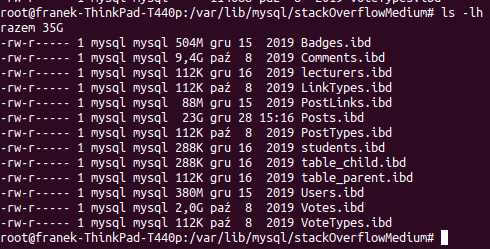
\includegraphics[scale = 0.43]{innodb-files.png}
	\label{fig:label}
\end{figure}

\begin{itemize}
	\item \textbf{Wsparcie dla transakcji. }
	\item \textbf{Blokowanie dostępu na poziomie rekordów. } Dostęp do tabel InnoDB jest blokowany za pomocą mechanizmy MVCC (Multi-Versioned Concurrency Control), który w przeciwieństwie do MyISAM blokuje pojedyncze rekordy, zamiast całej tabeli. Wprowadzenie tej zmiany znacząco zwiększyło wydajność równoległych operacji modyfikujące dane w tabeli.
	\item \textbf{Wsparcie dla kluczy obcych.}
\end{itemize}

\subsubsection{CSV Storage Engine}
Silnik CSV Storage Engine przechowuje dane tabeli w plikach tekstowych w formacie csv z wartościami rozdzielonymi przecinkami.Ten silnik może być przydatny, jeżeli chcemy nasze dane przechowywać w formacie csv, ale posiada wiele ograniczeń, dlatego nie jest zalecane jego stosowanie w większości przypadków.

\begin{itemize}
	\item \textbf{Brak wsparcia dla indeksów.}
	\item \textbf{Brak możliwości przechowywania wartości \textit{null}.}
	\item \textbf{Brak wsparcia dla partycjonowania.}
\end{itemize}

\subsubsection{Memory}
Tabele z silnikiem Memory są tabelami, których dane przechowywane są w pamięci, a nie na dysku twardym. Dane przechowywane w tabeli są ulotne i zostają usunięte w momencie restartu serwera (struktura tabeli zostaje zachowana). Z powodu przechowywania w pamięci są o rząd wielkości szybsze od standardowych silników baz danych, ale ze względu na swoją ulotność nie powinny przechowywać istotnych danych dla aplikacji. Poniżej wymieniłem kilka przypadków użyca tabeli z silnikiem Memory. 
\begin{itemize}
	\item Pamięć podręczna dla często odczytywanych danych, która jest wczytywana w momencie startu serwera.
	\item Buforowanie wyników agregowanych danych z często wykonywanych zapytań.
	\item Przechowywanie wyników pośrednich z zapytań.
	\item MySQL używa tabeli Memory do wewnętrznego przetwarzania zapytań wymagających tabeli tymczasowych do przechowywania wyników pośrednich.
\end{itemize}
Niżej przedstawiłem kilka podstawowych własności tabeli Memory.
\begin{itemize}
	\item \textbf{Indeksy Hash} Tabele Memory obsługują indeksy Hash (opisane w rozdziale dotyczącym indeksów).
	\item \textbf{Blokowanie na poziomie tabeli.} Podobnie jak tabele MyISAM, w momencie modyfikowania danych blokowana jest cała tabela.
	\item \textbf{Brak obsługi typów TEXT oraz BLOB}. Tabele nie obsługują typów TEXT. Przechowywanie teksu możliwe jest w kolumnach VARCHAR o stałej zdefiniowanej wielkości, co prowadzi do marnotrawienia pamięci.
\end{itemize}
